%!TEX root = ../../thesis.tex
\chapter{Overview}

Brain tumor segmentation and identification are the focus of this research. To assess the anatomy of the brain, MRI or CT scans are frequently used. MRI scanned image is utilized throughout this investigation. The MRI scan is less intrusive than the CT scan for assessing a patient's health.

Magnetic fields and radio waves are at the core of this technology. Numerous algorithms have been developed to detect brain tumors. However, detection and extraction may be impeded.

This research includes two alternative segmentation approaches. Fuzzy C mean and K-means clustering techniques. For this reason, it offers an accurate tumor segmentation result.
Any part of the body may become a tumor if its tissues develop out of control.
Depending on its location, a tumor could be either primary or secondary \ref{fig:human_brain_parts}.
The word "primary" refers to everything that has a beginning. It is stated to be
secondary if a piece of the tumor spreads and develops in a new place.
CSF is generally altered by brain tumors (Cerebral Spinal Fluid) (Cerebral Spinal
Fluid). Strokes are caused by it.

\begin{figure}
    \centering
    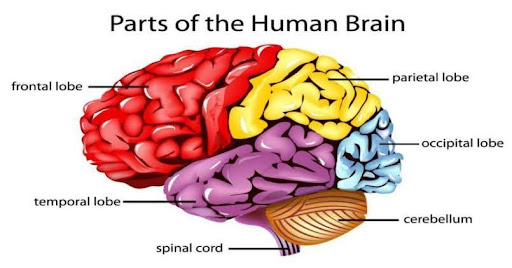
\includegraphics[width=0.60\textwidth]{Img/chap-03/human_brain_parts.jpg}
    \caption{Human Brain Parts.}
    \label{fig:human_brain_parts}
\end{figure}

Instead of treating cancer, the doctor offers treatment for strokes. Consequently,
early detection of malignancies is important to the success of this treatment.
If found early enough, a brain tumor may be more efficiently treated, and the
patient's life expectancy may be prolonged.
That will increase the life of the gadget by about a year or two.
T-cells and B-cells are the two most prevalent forms of cancer cells. Both the
frequency and the severity of these tumors suggest their malignancy. Mass tumors
make the detection of malignant tumors more a particular tumor location and detect
malignancy in the brain using this technology.
Treatment in most situations is focused on removing or eradicating the tumor \ref{fig:left_and_right_brain}.

\begin{figure}
    \centering
    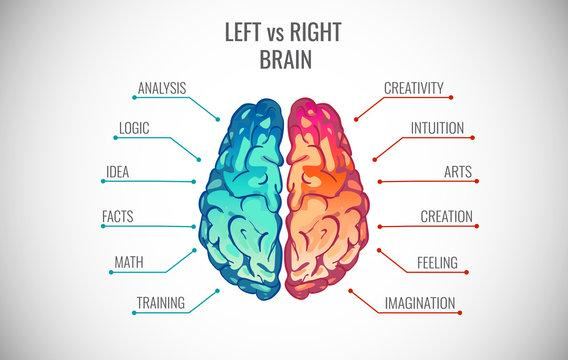
\includegraphics[width=0.60\textwidth]{Img/Chap-01/4.jpg}
    \caption{Left Brain \& Right Brain.}
    \label{fig:left_and_right_brain}
\end{figure}

If discovered and treated early, most brain tumors may be cured.
The number of persons with brain tumors is growing at an alarming pace due to
their incapacity to speak.

This project's major purpose is to enable people to learn to build tools. A tool that
can tell people whether or not they are in danger of having a brain tumor, as
well as how great of a risk they have. Java is the programming language utilized to develop the detecting system.
    
As a penultimate step, we are designing technologies that can assess the tumor's
morphology and stage from a particular tumor location.
The illustrations below illustrate the different parts of the brain. Two types of the
nervous system are the central and peripheral nervous systems.
Most of the nervous system consists of the brain and spinal cord (CNS). The spiral
cord and skull are both vital nerves (PNS) \ref{fig:brain_tumor_example} of the Peripheral Nervous System.

\begin{figure}
    \centering
    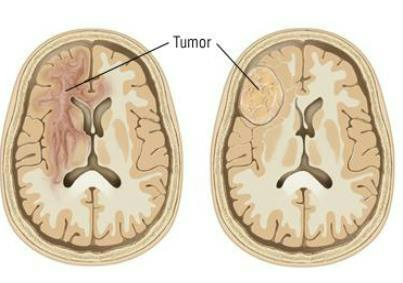
\includegraphics[width=0.60\textwidth]{Img/Chap-01/5.jpg}
    \caption{Brain Tumor Example.}
    \label{fig:brain_tumor_example}
\end{figure}

The spinal cord and the brain give rise to the spinal and cranial nerves, respectively.
Previously, it described how the Peripheral Nervous Systems (PNS) regulate a
variety of biological activities, including respiration, digestion, heart rate, and
hormone secretion (PNS). 

It consists of the brainstem, cerebrum, and cerebellum as its three principal regions. The cerebrum and cerebellum are connected to the spinal cord via the brain stem. The cerebrum is the biggest area of the brain. It has a right as well as a left hemisphere. The cerebrum oversees all elements of a person's
mental and emotional health, as well as their ability to communicate

The cerebellum is the brain's subsidiary structure. The cerebrum must coordinate the movement of the muscles. Many regions of the brainstem include the midbrain, Pons, and medulla. The brain stem is responsible for numerous autonomic functions of the body, such as waking and sleeping cycles, digestion,
sneezing, heart rate, breathing, body temperature, coughing, vomiting, and swallowing. The folds on the surface of the cerebrum are referred to as the cortex.

Of the 100 billion nerve cells in the brain, the cortex contains around 70\% of them. Grey matter, the component that gives the cortex its gray-brown tone, is composed of nerve cell bodies. As seen in \ref{fig:human_brain_parts}, the white matter is composed of the long, linked fibers known as axons found in the cortex.

 The corpus callosum links the brain's two hemispheres. It facilitates the flow of communication between the two parties. Each hemisphere of the brain is responsible for controlling a distinct side of the body. Weakness or paralysis of the left arm or leg could result from a tumor on the right side of the brain. The left hemisphere of the brain is responsible for thinking, mathematics, speaking, and writing. The right hemisphere oversaw imagination, three-dimensional ability, creativity, and musical aptitude. The left hemisphere dominates hand use and language in around 92\% of individuals \cite{ma82}.

\section{Scope}

Due to its soft tissue contrast and non-invasiveness, MR imaging is a popular option for significant medical imaging of the brain. MR imaging can also be employed to monitor how the size of a brain tumor varies as a result of treatment. A better method for separating tumors is required. Quantifying tumor volumes using MR images is currently impossible as a result of commonly accepted clinical practice procedures.

\section{Objective}

The objectives of this work can be summarized in the set of the following points:

\begin{enumerate}[a)]
    \item The primary goal is to create a framework that will assist clinical specialists in cross-confirming their predicted brain tumor type analysis results.
    \item Because the current diagnosis process is time-consuming, labor-intensive, and expensive, this deep learning-based tool can detect tumor growth and predict stage.
    \item Because this is an automated tool that uses image processing and AI, it reduces the amount of human effort required to predict the existence of tumor type from images.
\end{enumerate}

\section{Need}

People who have had past brain tumors are more likely to get a new one. If you have two or more close relatives who have brain tumors, your risk of developing one is increased. Even though it is very unusual, members of the same family can be born with a disease that renders the brain more susceptible to growing a tumor. Around 5\% of all brain tumors may have a genetic component.

\section{Motivation}

\begin{enumerate}[a)]
    \item It's obvious that a technique for accurately segmenting tumors would be valuable. Quantitating tumor regions using MR images is currently impossible due to a lack of well-acknowledged clinical practice methods.
    \item It is our major goal in this research to detect if there is a Brain tumor or not and classify the tumor into its types if the tumor is present, such as Glioma, Meningioma, and Pituitary.
\end{enumerate}
